\SourceLeaf{199}$AB = AE$, $ABE = AEB$; folglich ist nun aus der Voraussetzung $ACB = ABD$ sogleich
(Satz 1) $ACE = ABC = ABE = AEB$. Also ist $AC = AE = AB$ gegen die Voraussetzung.

\begin{center}
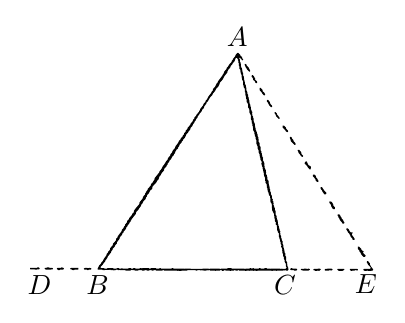
\begin{tikzpicture}[x=0.00498375cm,y=-0.00498375cm]
\fill[even odd rule] (835,623) -- (835,624) -- (838,627) -- (840,627) -- (841,626) -- (847,626) -- (848,625) -- (854,626) -- (855,625) -- (855,623) -- (854,622) -- (836,622) -- cycle
(803,623) -- (803,624) -- (807,627) -- (816,627) -- (821,624) -- (820,622) -- (804,622) -- cycle
(771,625) -- (772,626) -- (782,626) -- (783,625) -- (788,626) -- (790,625) -- (791,623) -- (788,621) -- (778,621) -- (777,622) -- (773,622) -- (771,624) -- cycle
(761,623) -- (759,621) -- (754,621) -- (753,622) -- (744,622) -- (742,623) -- (742,625) -- (746,626) -- (747,627) -- (751,627) -- (752,626) -- (757,627) -- (759,625) -- (760,625) -- cycle
(710,623) -- (711,625) -- (714,625) -- (715,626) -- (730,626) -- (733,624) -- (733,623) -- (731,621) -- (729,621) -- (728,622) -- (725,622) -- (724,621) -- (719,621) -- (718,622) -- (711,622) -- cycle
(683,622) -- (683,623) -- (685,625) -- (692,625) -- (693,626) -- (699,626) -- (701,624) -- (701,623) -- (698,621) -- (689,621) -- (688,620) -- (686,620) -- cycle
(158,621) -- (158,622) -- (160,624) -- (166,624) -- (167,625) -- (169,625) -- (170,624) -- (175,624) -- (177,622) -- (176,620) -- (174,620) -- (173,619) -- (171,619) -- (170,620) -- (162,619) -- cycle
(123,621) -- (124,623) -- (126,623) -- (130,625) -- (133,625) -- (134,624) -- (143,624) -- (144,623) -- (144,620) -- (143,619) -- (127,619) -- cycle
(107,621) -- (105,619) -- (101,618) -- (100,619) -- (91,619) -- (89,621) -- (89,622) -- (93,625) -- (96,625) -- (97,624) -- (104,624) -- (106,623) -- cycle
(58,620) -- (58,621) -- (61,624) -- (74,624) -- (75,623) -- (78,623) -- (79,622) -- (79,621) -- (77,619) -- (70,619) -- (69,618) -- (64,618) -- (63,619) -- (59,619) -- cycle
(45,620) -- (43,618) -- (40,618) -- (39,619) -- (22,619) -- (21,620) -- (21,622) -- (22,623) -- (33,623) -- (34,624) -- (38,624) -- (39,623) -- (44,623) -- (45,622) -- cycle
(879,602) -- (878,603) -- (878,606) -- (880,608) -- (881,611) -- (887,617) -- (888,620) -- (886,622) -- (871,622) -- (869,624) -- (869,625) -- (873,627) -- (877,627) -- (878,626) -- (880,626) -- (881,627) -- (889,627) -- (890,626) -- (893,626) -- (894,625) -- (894,623) -- (888,615) -- (886,611) -- (886,608) -- (881,602) -- cycle
(856,565) -- (855,566) -- (855,571) -- (859,575) -- (859,577) -- (863,582) -- (863,584) -- (869,591) -- (873,591) -- (875,589) -- (875,588) -- (868,581) -- (870,577) -- (866,575) -- (864,573) -- (864,571) -- (858,565) -- cycle
(827,519) -- (826,520) -- (826,522) -- (829,526) -- (830,529) -- (834,533) -- (834,535) -- (836,537) -- (837,540) -- (841,544) -- (841,546) -- (843,548) -- (846,548) -- (847,547) -- (847,545) -- (840,535) -- (840,532) -- (842,531) -- (842,529) -- (837,529) -- (835,527) -- (832,521) -- (830,519) -- cycle
(805,483) -- (804,484) -- (804,487) -- (806,489) -- (806,491) -- (809,495) -- (809,497) -- (815,504) -- (815,505) -- (817,507) -- (819,507) -- (821,505) -- (821,503) -- (819,501) -- (818,498) -- (814,494) -- (814,492) -- (812,490) -- (810,485) -- (808,483) -- cycle
(784,450) -- (783,451) -- (783,454) -- (787,459) -- (787,462) -- (789,464) -- (789,466) -- (793,470) -- (796,470) -- (797,469) -- (797,465) -- (793,461) -- (793,459) -- (790,453) -- (788,451) -- cycle
(761,414) -- (760,416) -- (762,420) -- (764,422) -- (765,425) -- (770,432) -- (773,432) -- (775,430) -- (775,428) -- (770,423) -- (764,414) -- cycle
(742,382) -- (741,383) -- (741,386) -- (747,393) -- (748,397) -- (751,400) -- (754,401) -- (755,400) -- (755,397) -- (753,395) -- (752,392) -- (749,389) -- (748,385) -- (745,382) -- cycle
(723,348) -- (720,352) -- (720,354) -- (726,360) -- (729,365) -- (733,369) -- (734,369) -- (735,368) -- (736,362) -- (733,359) -- (731,359) -- (729,357) -- (729,355) -- (727,353) -- (726,350) -- (724,348) -- cycle
(703,319) -- (702,321) -- (704,324) -- (704,326) -- (709,332) -- (709,333) -- (713,337) -- (714,337) -- (716,335) -- (716,334) -- (712,330) -- (711,325) -- (706,319) -- cycle
(683,286) -- (682,287) -- (682,289) -- (683,290) -- (685,297) -- (694,306) -- (696,306) -- (697,304) -- (695,300) -- (692,297) -- (691,294) -- (688,291) -- (687,288) -- (685,286) -- cycle
(664,257) -- (664,262) -- (670,268) -- (672,272) -- (676,274) -- (678,272) -- (678,271) -- (672,264) -- (672,262) -- (667,257) -- cycle
(644,223) -- (643,225) -- (646,229) -- (647,233) -- (654,240) -- (655,240) -- (656,239) -- (656,237) -- (649,228) -- (649,226) -- (646,223) -- cycle
(625,192) -- (624,193) -- (624,196) -- (626,198) -- (630,206) -- (634,210) -- (636,210) -- (637,209) -- (637,207) -- (632,201) -- (631,197) -- (627,192) -- cycle
(606,161) -- (605,162) -- (605,166) -- (606,168) -- (610,172) -- (613,177) -- (616,180) -- (618,180) -- (619,179) -- (619,177) -- (617,173) -- (613,170) -- (613,167) -- (609,163) -- (609,162) -- (608,161) -- cycle
(586,129) -- (585,130) -- (585,133) -- (587,135) -- (589,139) -- (589,141) -- (593,144) -- (594,147) -- (596,149) -- (598,149) -- (599,148) -- (599,146) -- (598,144) -- (594,141) -- (594,137) -- (592,135) -- (591,132) -- (588,129) -- cycle
(568,100) -- (567,102) -- (571,111) -- (573,113) -- (573,114) -- (579,120) -- (580,120) -- (581,119) -- (581,117) -- (577,109) -- (572,104) -- (572,102) -- cycle
(551,72) -- (549,72) -- (545,76) -- (542,82) -- (537,88) -- (537,90) -- (534,93) -- (534,95) -- (529,100) -- (524,108) -- (521,111) -- (521,113) -- (515,120) -- (514,124) -- (512,126) -- (511,129) -- (499,145) -- (499,147) -- (496,150) -- (492,158) -- (488,162) -- (486,166) -- (486,168) -- (483,171) -- (482,174) -- (475,183) -- (471,191) -- (468,194) -- (467,197) -- (463,201) -- (461,206) -- (454,215) -- (454,217) -- (452,219) -- (451,222) -- (445,229) -- (443,233) -- (439,237) -- (439,239) -- (436,242) -- (435,246) -- (429,253) -- (429,255) -- (422,263) -- (421,266) -- (417,270) -- (417,273) -- (413,277) -- (413,279) -- (410,282) -- (409,285) -- (405,289) -- (404,292) -- (400,296) -- (398,301) -- (391,310) -- (390,314) -- (384,321) -- (382,326) -- (378,330) -- (378,333) -- (372,340) -- (371,344) -- (368,347) -- (362,357) -- (359,360) -- (355,368) -- (350,374) -- (350,376) -- (338,391) -- (337,396) -- (335,398) -- (333,402) -- (329,406) -- (328,410) -- (320,419) -- (320,421) -- (316,426) -- (316,428) -- (314,430) -- (314,432) -- (308,439) -- (308,442) -- (300,452) -- (299,454) -- (299,457) -- (288,470) -- (285,475) -- (285,478) -- (281,482) -- (280,485) -- (273,493) -- (273,495) -- (268,500) -- (268,503) -- (263,509) -- (263,511) -- (259,516) -- (259,518) -- (255,522) -- (254,526) -- (244,539) -- (244,541) -- (240,545) -- (240,549) -- (232,558) -- (232,561) -- (225,569) -- (224,574) -- (220,578) -- (219,581) -- (216,584) -- (215,588) -- (209,596) -- (206,602) -- (203,605) -- (201,609) -- (197,613) -- (193,621) -- (193,623) -- (194,624) -- (205,624) -- (206,625) -- (225,624) -- (226,625) -- (233,625) -- (234,626) -- (236,625) -- (239,625) -- (240,624) -- (244,624) -- (245,625) -- (248,625) -- (249,624) -- (251,625) -- (263,625) -- (264,626) -- (276,626) -- (280,624) -- (282,625) -- (287,625) -- (288,626) -- (296,626) -- (297,625) -- (305,625) -- (306,626) -- (312,626) -- (313,625) -- (317,625) -- (318,626) -- (324,626) -- (325,625) -- (330,625) -- (331,626) -- (335,626) -- (336,625) -- (341,625) -- (342,626) -- (358,626) -- (359,625) -- (361,625) -- (362,626) -- (395,626) -- (396,627) -- (398,627) -- (399,626) -- (401,627) -- (406,627) -- (407,626) -- (421,626) -- (422,625) -- (442,625) -- (443,626) -- (446,626) -- (447,625) -- (454,625) -- (455,626) -- (457,625) -- (459,626) -- (461,625) -- (463,626) -- (470,626) -- (471,625) -- (474,626) -- (475,625) -- (478,625) -- (479,626) -- (492,626) -- (493,627) -- (495,626) -- (504,626) -- (505,625) -- (508,625) -- (510,627) -- (512,627) -- (516,625) -- (518,625) -- (519,626) -- (529,626) -- (530,627) -- (532,627) -- (533,626) -- (540,626) -- (541,625) -- (543,625) -- (544,626) -- (549,626) -- (550,625) -- (552,625) -- (553,626) -- (568,626) -- (569,627) -- (571,627) -- (572,626) -- (579,626) -- (580,627) -- (582,626) -- (589,626) -- (590,627) -- (592,626) -- (595,626) -- (596,627) -- (599,627) -- (600,626) -- (635,626) -- (636,627) -- (638,627) -- (639,626) -- (646,626) -- (648,627) -- (649,626) -- (666,626) -- (667,625) -- (669,626) -- (671,625) -- (673,626) -- (677,626) -- (678,625) -- (679,622) -- (678,621) -- (678,618) -- (676,615) -- (675,605) -- (673,602) -- (673,591) -- (671,589) -- (671,583) -- (669,581) -- (668,573) -- (667,572) -- (667,569) -- (666,568) -- (666,562) -- (664,559) -- (664,552) -- (662,550) -- (661,544) -- (660,543) -- (660,539) -- (658,535) -- (658,531) -- (657,530) -- (658,526) -- (656,524) -- (656,520) -- (655,519) -- (654,513) -- (653,512) -- (653,509) -- (652,508) -- (652,502) -- (651,501) -- (651,498) -- (649,494) -- (648,486) -- (646,484) -- (646,475) -- (644,472) -- (644,467) -- (642,465) -- (642,462) -- (640,458) -- (641,455) -- (640,454) -- (640,450) -- (638,448) -- (639,445) -- (637,443) -- (636,435) -- (634,432) -- (634,428) -- (632,424) -- (632,419) -- (631,418) -- (630,410) -- (629,409) -- (629,406) -- (628,405) -- (628,398) -- (625,394) -- (625,388) -- (624,387) -- (624,384) -- (621,380) -- (622,378) -- (622,376) -- (621,375) -- (621,370) -- (619,368) -- (619,366) -- (618,365) -- (617,352) -- (616,351) -- (616,349) -- (614,347) -- (614,344) -- (613,343) -- (614,339) -- (612,337) -- (612,334) -- (611,333) -- (611,328) -- (610,327) -- (610,323) -- (608,321) -- (608,312) -- (605,308) -- (605,301) -- (603,299) -- (602,287) -- (600,284) -- (600,280) -- (599,279) -- (599,277) -- (598,276) -- (598,274) -- (595,267) -- (595,263) -- (594,262) -- (594,259) -- (593,258) -- (593,253) -- (590,246) -- (590,239) -- (589,238) -- (589,235) -- (587,232) -- (587,229) -- (586,228) -- (586,225) -- (587,223) -- (585,221) -- (585,219) -- (583,215) -- (583,210) -- (582,209) -- (582,205) -- (580,202) -- (580,199) -- (579,198) -- (579,193) -- (578,192) -- (578,189) -- (577,188) -- (577,185) -- (576,184) -- (576,179) -- (574,176) -- (574,172) -- (572,169) -- (571,159) -- (570,158) -- (570,155) -- (568,151) -- (568,147) -- (567,146) -- (567,143) -- (566,142) -- (565,133) -- (563,129) -- (563,123) -- (562,122) -- (560,111) -- (558,108) -- (557,98) -- (555,94) -- (555,89) -- (553,86) -- (555,84) -- (561,91) -- (563,90) -- (563,88) -- (561,86) -- (561,83) -- (556,79) -- (556,77) -- cycle
(547,85) -- (550,88) -- (550,91) -- (551,92) -- (551,97) -- (553,100) -- (552,103) -- (554,107) -- (554,113) -- (556,115) -- (556,119) -- (557,120) -- (557,123) -- (559,127) -- (560,137) -- (561,138) -- (561,141) -- (563,144) -- (563,153) -- (564,154) -- (565,160) -- (567,162) -- (567,164) -- (568,165) -- (568,172) -- (569,173) -- (569,180) -- (570,181) -- (570,185) -- (571,186) -- (571,189) -- (572,190) -- (572,197) -- (574,199) -- (576,203) -- (576,211) -- (578,213) -- (578,215) -- (579,216) -- (579,223) -- (583,231) -- (583,241) -- (585,244) -- (585,247) -- (586,248) -- (585,251) -- (587,253) -- (587,258) -- (588,259) -- (588,262) -- (589,263) -- (589,269) -- (592,274) -- (592,279) -- (593,280) -- (593,283) -- (595,286) -- (595,291) -- (597,294) -- (597,303) -- (600,310) -- (600,315) -- (603,321) -- (603,326) -- (605,330) -- (605,334) -- (606,335) -- (606,338) -- (607,339) -- (607,343) -- (609,347) -- (611,349) -- (611,351) -- (610,352) -- (610,356) -- (611,357) -- (611,360) -- (613,363) -- (613,368) -- (614,369) -- (614,372) -- (615,373) -- (615,376) -- (616,377) -- (616,382) -- (617,383) -- (617,386) -- (619,390) -- (619,397) -- (621,399) -- (620,403) -- (623,406) -- (624,415) -- (625,416) -- (625,419) -- (626,420) -- (625,421) -- (626,422) -- (626,425) -- (628,428) -- (629,434) -- (632,437) -- (633,452) -- (636,456) -- (637,472) -- (642,482) -- (643,493) -- (644,494) -- (644,500) -- (647,504) -- (646,508) -- (650,512) -- (649,514) -- (649,516) -- (650,517) -- (650,524) -- (651,525) -- (652,529) -- (654,531) -- (654,540) -- (655,541) -- (656,546) -- (658,548) -- (657,551) -- (659,554) -- (659,559) -- (661,561) -- (660,565) -- (663,571) -- (663,573) -- (662,574) -- (663,576) -- (663,581) -- (665,584) -- (665,589) -- (667,592) -- (667,596) -- (669,600) -- (669,604) -- (672,609) -- (672,615) -- (674,619) -- (671,622) -- (663,622) -- (662,621) -- (660,622) -- (658,622) -- (657,621) -- (634,621) -- (632,622) -- (631,621) -- (624,621) -- (623,620) -- (618,620) -- (617,621) -- (608,621) -- (607,620) -- (604,620) -- (603,621) -- (591,621) -- (590,620) -- (584,621) -- (583,620) -- (581,620) -- (580,621) -- (570,621) -- (569,622) -- (567,622) -- (566,621) -- (534,621) -- (533,620) -- (524,620) -- (523,621) -- (508,621) -- (507,622) -- (504,622) -- (503,621) -- (479,621) -- (478,622) -- (476,622) -- (475,621) -- (461,621) -- (460,622) -- (430,622) -- (429,621) -- (417,621) -- (415,622) -- (414,621) -- (386,621) -- (385,620) -- (382,620) -- (381,621) -- (354,621) -- (353,620) -- (351,620) -- (350,621) -- (342,621) -- (341,620) -- (329,620) -- (328,621) -- (324,621) -- (323,620) -- (307,620) -- (306,621) -- (304,620) -- (301,620) -- (300,621) -- (289,621) -- (288,620) -- (284,620) -- (283,621) -- (278,621) -- (277,620) -- (272,620) -- (271,621) -- (256,621) -- (255,620) -- (253,621) -- (248,621) -- (247,620) -- (242,620) -- (241,621) -- (233,621) -- (232,620) -- (218,620) -- (217,621) -- (210,621) -- (209,620) -- (202,620) -- (200,618) -- (200,617) -- (206,611) -- (206,610) -- (212,603) -- (213,600) -- (217,595) -- (219,590) -- (227,580) -- (227,578) -- (231,573) -- (231,571) -- (236,566) -- (238,561) -- (242,557) -- (242,554) -- (249,545) -- (249,543) -- (252,538) -- (255,535) -- (255,533) -- (259,529) -- (259,527) -- (265,520) -- (266,516) -- (269,513) -- (269,511) -- (273,507) -- (274,504) -- (277,501) -- (277,499) -- (279,497) -- (279,496) -- (290,482) -- (291,477) -- (297,471) -- (297,470) -- (303,462) -- (304,458) -- (307,455) -- (310,449) -- (315,444) -- (316,440) -- (318,438) -- (319,434) -- (323,430) -- (327,422) -- (331,419) -- (332,417) -- (332,413) -- (343,401) -- (344,398) -- (348,394) -- (350,387) -- (353,384) -- (356,378) -- (362,371) -- (362,368) -- (363,366) -- (368,361) -- (369,358) -- (371,356) -- (371,354) -- (375,349) -- (376,346) -- (380,342) -- (383,336) -- (387,332) -- (387,330) -- (390,327) -- (390,324) -- (393,321) -- (393,319) -- (398,315) -- (398,312) -- (400,310) -- (402,305) -- (407,300) -- (407,298) -- (410,295) -- (411,292) -- (415,288) -- (419,279) -- (423,275) -- (425,271) -- (428,268) -- (430,262) -- (434,258) -- (436,253) -- (439,250) -- (439,248) -- (443,243) -- (444,240) -- (447,237) -- (448,233) -- (451,230) -- (453,226) -- (457,222) -- (459,217) -- (463,213) -- (465,207) -- (470,201) -- (470,199) -- (473,196) -- (480,184) -- (485,179) -- (486,176) -- (492,169) -- (495,163) -- (500,158) -- (503,152) -- (504,148) -- (511,140) -- (515,132) -- (523,122) -- (523,120) -- (526,114) -- (530,110) -- (532,105) -- (536,101) -- (537,98) -- (541,94) -- (544,86) -- (545,85) -- cycle;
\node[inner sep=0pt] at (548,32) {$A$};
\node[inner sep=0pt] at (45,662) {$D$};
\node[inner sep=0pt] at (193,662) {$B$};
\node[inner sep=0pt] at (670,663) {$C$};
\node[inner sep=0pt] at (876,661) {$E$};
\end{tikzpicture}
\\[3pt]Fig. 3.
\end{center}

\emph{6. Lehrsatz.} Kein Winkel eines Dreiecks kann grösser sein als der Nebenwinkel
eines andern Winkels in demselben Dreieck.

$ACB$ kann nicht grösser sein als $ABD$.

\textls{Beweis.} Man beschreibe eine Kegelfläche, Axe $CB$, Spitze $C$, Winkel dem $ABD$
gleich. Wäre nun $ABD$ kleiner als $ACB$, so würde die Linie $CA$ ausserhalb des
Kegels liegen (Definition) und da $B$, als Punkt in der Axe, innerhalb liegt, so
muss die Gerade $AB$ die Kegelfläche schneiden. Das geschehe in $E$. Es wird also
$ECB = EBD$, welches nicht möglich ist (Satz 5).


 

\begin{center}
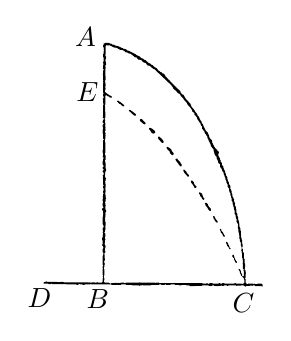
\begin{tikzpicture}[x=0.00557554cm,y=-0.00557554cm]
\fill[even odd rule] (184,47) -- (183,48) -- (183,51) -- (182,52) -- (182,55) -- (184,58) -- (183,60) -- (184,62) -- (184,65) -- (183,66) -- (183,71) -- (182,72) -- (182,78) -- (183,79) -- (183,89) -- (182,90) -- (183,97) -- (182,98) -- (182,105) -- (183,106) -- (183,109) -- (182,110) -- (182,117) -- (181,118) -- (182,120) -- (182,131) -- (183,132) -- (182,134) -- (182,136) -- (183,137) -- (182,139) -- (182,159) -- (183,160) -- (183,162) -- (182,163) -- (182,167) -- (183,168) -- (183,172) -- (181,174) -- (182,176) -- (182,184) -- (183,185) -- (183,187) -- (182,188) -- (182,214) -- (181,216) -- (184,219) -- (181,225) -- (181,227) -- (183,229) -- (183,231) -- (181,233) -- (181,238) -- (182,239) -- (182,243) -- (181,244) -- (181,247) -- (182,249) -- (181,250) -- (181,252) -- (182,253) -- (182,264) -- (184,266) -- (184,267) -- (182,269) -- (182,290) -- (181,291) -- (181,296) -- (182,297) -- (182,304) -- (181,306) -- (183,308) -- (183,310) -- (182,311) -- (182,315) -- (181,316) -- (181,323) -- (183,326) -- (183,328) -- (181,330) -- (181,332) -- (183,334) -- (183,336) -- (181,338) -- (181,340) -- (183,342) -- (183,347) -- (181,349) -- (182,351) -- (182,353) -- (181,354) -- (182,356) -- (182,369) -- (183,370) -- (183,372) -- (182,373) -- (182,377) -- (183,378) -- (183,383) -- (182,384) -- (182,387) -- (183,388) -- (183,390) -- (182,391) -- (182,396) -- (181,397) -- (182,399) -- (182,401) -- (181,402) -- (181,407) -- (182,408) -- (182,410) -- (181,411) -- (181,418) -- (183,420) -- (183,421) -- (180,424) -- (180,427) -- (182,430) -- (182,435) -- (183,436) -- (182,438) -- (182,442) -- (181,443) -- (181,459) -- (183,463) -- (183,466) -- (181,470) -- (181,473) -- (182,474) -- (182,476) -- (181,477) -- (182,483) -- (181,485) -- (182,487) -- (180,491) -- (180,496) -- (181,497) -- (181,505) -- (180,506) -- (180,508) -- (182,510) -- (182,512) -- (183,513) -- (183,514) -- (181,516) -- (181,523) -- (183,525) -- (182,531) -- (181,532) -- (181,552) -- (182,553) -- (182,555) -- (181,556) -- (181,560) -- (182,561) -- (181,563) -- (181,575) -- (182,576) -- (182,578) -- (181,579) -- (182,581) -- (182,583) -- (181,584) -- (181,591) -- (179,593) -- (171,593) -- (170,592) -- (167,592) -- (166,593) -- (163,593) -- (162,592) -- (157,592) -- (156,593) -- (153,593) -- (151,592) -- (149,593) -- (148,592) -- (92,592) -- (91,591) -- (77,592) -- (76,591) -- (54,591) -- (52,590) -- (51,591) -- (47,592) -- (46,594) -- (47,595) -- (57,595) -- (58,596) -- (62,596) -- (63,595) -- (65,595) -- (66,596) -- (98,596) -- (99,597) -- (121,597) -- (122,598) -- (124,598) -- (127,596) -- (129,596) -- (130,597) -- (135,597) -- (136,598) -- (139,598) -- (140,597) -- (152,597) -- (153,596) -- (155,596) -- (156,597) -- (201,597) -- (202,598) -- (214,598) -- (215,597) -- (216,598) -- (222,598) -- (223,597) -- (234,597) -- (235,598) -- (248,598) -- (249,599) -- (263,599) -- (265,600) -- (266,599) -- (270,599) -- (271,598) -- (273,599) -- (291,599) -- (292,598) -- (309,598) -- (310,597) -- (314,597) -- (315,598) -- (322,598) -- (323,597) -- (325,597) -- (326,598) -- (335,598) -- (336,597) -- (342,597) -- (344,596) -- (346,598) -- (355,598) -- (356,599) -- (360,599) -- (361,598) -- (371,598) -- (372,599) -- (378,599) -- (381,601) -- (388,601) -- (389,600) -- (391,601) -- (393,600) -- (407,600) -- (408,599) -- (422,599) -- (423,600) -- (430,600) -- (431,599) -- (434,599) -- (435,600) -- (440,600) -- (441,601) -- (444,601) -- (445,600) -- (450,600) -- (451,599) -- (453,600) -- (457,600) -- (458,599) -- (464,599) -- (465,600) -- (467,600) -- (468,599) -- (485,599) -- (486,600) -- (502,599) -- (507,602) -- (509,600) -- (517,600) -- (518,599) -- (523,600) -- (524,599) -- (527,599) -- (530,601) -- (533,601) -- (534,600) -- (538,601) -- (540,600) -- (541,601) -- (544,601) -- (546,602) -- (546,598) -- (543,595) -- (535,595) -- (534,596) -- (528,596) -- (527,595) -- (525,596) -- (523,595) -- (513,595) -- (512,596) -- (510,596) -- (507,593) -- (507,585) -- (506,584) -- (506,582) -- (507,581) -- (507,573) -- (508,571) -- (507,570) -- (507,566) -- (505,563) -- (505,561) -- (506,560) -- (505,558) -- (506,556) -- (506,550) -- (505,549) -- (505,540) -- (503,537) -- (503,525) -- (501,523) -- (501,517) -- (499,515) -- (499,512) -- (500,511) -- (500,505) -- (499,504) -- (499,496) -- (498,495) -- (498,492) -- (496,488) -- (497,486) -- (496,484) -- (496,475) -- (495,474) -- (495,469) -- (493,465) -- (493,459) -- (492,458) -- (492,454) -- (491,453) -- (491,450) -- (490,449) -- (490,444) -- (488,440) -- (488,436) -- (486,433) -- (486,426) -- (485,425) -- (485,421) -- (482,415) -- (483,412) -- (482,411) -- (482,409) -- (480,407) -- (481,404) -- (477,396) -- (477,392) -- (475,388) -- (475,384) -- (474,383) -- (474,381) -- (472,379) -- (472,372) -- (469,368) -- (469,365) -- (466,359) -- (465,352) -- (462,348) -- (462,345) -- (460,342) -- (460,338) -- (458,336) -- (458,334) -- (456,331) -- (456,328) -- (453,325) -- (453,320) -- (450,317) -- (450,314) -- (448,312) -- (448,309) -- (445,304) -- (445,298) -- (446,297) -- (446,294) -- (445,294) -- (436,284) -- (431,274) -- (430,268) -- (425,263) -- (423,256) -- (421,253) -- (421,251) -- (416,246) -- (411,236) -- (410,232) -- (407,229) -- (406,225) -- (404,223) -- (400,214) -- (397,211) -- (397,209) -- (392,203) -- (390,199) -- (383,191) -- (383,188) -- (381,186) -- (381,185) -- (370,173) -- (365,164) -- (363,164) -- (359,160) -- (358,156) -- (354,152) -- (353,152) -- (335,134) -- (335,133) -- (332,130) -- (331,130) -- (329,128) -- (329,127) -- (324,122) -- (324,121) -- (320,116) -- (318,116) -- (315,113) -- (313,113) -- (310,110) -- (309,110) -- (304,104) -- (299,101) -- (295,97) -- (292,96) -- (289,93) -- (286,92) -- (278,85) -- (276,85) -- (273,82) -- (269,81) -- (265,77) -- (258,74) -- (256,72) -- (240,64) -- (238,64) -- (236,62) -- (232,60) -- (229,60) -- (227,58) -- (225,58) -- (217,54) -- (209,52) -- (207,50) -- (203,50) -- (201,48) -- (198,48) -- (195,46) -- (187,46) -- (186,47) -- cycle
(190,51) -- (192,52) -- (198,52) -- (208,57) -- (212,57) -- (213,58) -- (215,58) -- (217,60) -- (221,62) -- (225,62) -- (231,65) -- (234,68) -- (237,68) -- (240,70) -- (245,71) -- (255,79) -- (258,79) -- (262,84) -- (269,85) -- (273,90) -- (279,92) -- (284,98) -- (287,98) -- (289,99) -- (296,105) -- (299,106) -- (338,143) -- (338,144) -- (341,147) -- (342,150) -- (345,153) -- (346,153) -- (353,161) -- (356,162) -- (358,164) -- (359,167) -- (365,173) -- (365,174) -- (373,183) -- (374,186) -- (382,195) -- (385,200) -- (385,202) -- (390,206) -- (390,209) -- (396,216) -- (397,220) -- (404,230) -- (405,234) -- (408,237) -- (408,242) -- (413,248) -- (414,252) -- (417,255) -- (418,258) -- (420,260) -- (420,263) -- (422,266) -- (423,270) -- (425,272) -- (425,274) -- (427,277) -- (427,279) -- (429,283) -- (434,289) -- (434,293) -- (435,294) -- (436,299) -- (438,303) -- (441,306) -- (441,310) -- (443,313) -- (445,320) -- (449,323) -- (449,329) -- (453,334) -- (453,336) -- (455,340) -- (457,342) -- (457,345) -- (459,349) -- (459,352) -- (461,354) -- (461,357) -- (463,361) -- (463,364) -- (466,369) -- (466,374) -- (469,378) -- (470,386) -- (472,388) -- (472,393) -- (474,396) -- (474,399) -- (475,400) -- (475,406) -- (477,408) -- (478,416) -- (479,417) -- (479,420) -- (480,421) -- (481,427) -- (482,428) -- (482,436) -- (484,439) -- (485,446) -- (487,449) -- (486,453) -- (490,461) -- (489,467) -- (490,468) -- (491,479) -- (492,480) -- (492,484) -- (493,485) -- (493,493) -- (494,494) -- (494,498) -- (496,502) -- (496,509) -- (498,511) -- (498,517) -- (497,519) -- (498,520) -- (498,524) -- (499,525) -- (499,536) -- (500,537) -- (500,541) -- (501,542) -- (501,547) -- (500,549) -- (501,550) -- (501,561) -- (503,563) -- (502,565) -- (503,567) -- (503,577) -- (501,579) -- (499,578) -- (499,574) -- (496,569) -- (496,566) -- (495,564) -- (493,562) -- (491,562) -- (491,563) -- (494,568) -- (494,570) -- (497,577) -- (500,580) -- (500,581) -- (501,581) -- (503,583) -- (503,585) -- (504,586) -- (504,593) -- (502,595) -- (498,596) -- (497,595) -- (485,595) -- (484,594) -- (482,594) -- (481,595) -- (459,595) -- (458,594) -- (454,594) -- (453,595) -- (449,595) -- (448,594) -- (446,594) -- (445,595) -- (432,595) -- (431,594) -- (426,594) -- (422,596) -- (419,594) -- (417,595) -- (409,595) -- (408,594) -- (345,594) -- (344,593) -- (342,594) -- (310,594) -- (309,593) -- (303,593) -- (301,594) -- (300,593) -- (267,593) -- (266,592) -- (264,593) -- (234,593) -- (233,594) -- (231,594) -- (230,593) -- (222,593) -- (221,594) -- (218,594) -- (217,593) -- (215,594) -- (209,593) -- (208,594) -- (201,594) -- (200,595) -- (198,595) -- (195,593) -- (186,593) -- (184,591) -- (184,588) -- (185,587) -- (185,583) -- (184,582) -- (184,577) -- (185,576) -- (185,563) -- (184,562) -- (184,558) -- (185,557) -- (185,552) -- (186,551) -- (184,544) -- (186,542) -- (185,526) -- (187,524) -- (187,521) -- (186,520) -- (186,515) -- (187,514) -- (187,511) -- (188,510) -- (185,504) -- (186,502) -- (186,496) -- (187,495) -- (187,493) -- (186,492) -- (186,489) -- (187,488) -- (187,481) -- (185,479) -- (185,478) -- (186,477) -- (186,473) -- (188,471) -- (187,469) -- (188,455) -- (186,453) -- (186,451) -- (187,450) -- (186,445) -- (187,444) -- (187,439) -- (188,438) -- (187,436) -- (187,433) -- (189,431) -- (189,429) -- (187,425) -- (187,419) -- (188,418) -- (188,416) -- (187,415) -- (187,411) -- (186,410) -- (186,409) -- (188,407) -- (188,402) -- (189,401) -- (188,399) -- (188,394) -- (187,393) -- (187,386) -- (188,385) -- (188,382) -- (187,381) -- (187,376) -- (188,375) -- (188,369) -- (187,368) -- (187,364) -- (186,363) -- (186,362) -- (188,360) -- (188,357) -- (189,356) -- (186,351) -- (187,340) -- (189,337) -- (189,334) -- (188,333) -- (188,330) -- (187,329) -- (188,327) -- (188,321) -- (187,320) -- (187,317) -- (186,316) -- (186,314) -- (188,312) -- (188,303) -- (186,301) -- (186,298) -- (187,297) -- (187,273) -- (186,272) -- (186,266) -- (187,265) -- (187,259) -- (188,258) -- (187,256) -- (188,252) -- (186,250) -- (186,248) -- (188,245) -- (187,243) -- (187,240) -- (188,238) -- (186,236) -- (187,234) -- (187,228) -- (186,227) -- (186,224) -- (187,222) -- (185,220) -- (187,216) -- (187,203) -- (186,202) -- (186,200) -- (187,199) -- (186,195) -- (187,193) -- (186,192) -- (186,188) -- (187,187) -- (187,167) -- (189,165) -- (193,168) -- (195,168) -- (198,171) -- (201,171) -- (202,170) -- (202,169) -- (200,167) -- (197,166) -- (186,158) -- (187,152) -- (188,151) -- (187,149) -- (187,144) -- (188,143) -- (188,140) -- (187,139) -- (187,136) -- (186,135) -- (187,131) -- (188,130) -- (188,128) -- (187,127) -- (188,125) -- (188,123) -- (187,122) -- (187,105) -- (188,104) -- (187,98) -- (189,95) -- (188,89) -- (187,88) -- (188,82) -- (189,81) -- (189,79) -- (187,75) -- (187,73) -- (188,72) -- (188,65) -- (187,63) -- (188,62) -- (188,53) -- cycle
(478,529) -- (477,530) -- (477,534) -- (481,538) -- (481,541) -- (484,547) -- (486,548) -- (487,547) -- (487,545) -- (485,543) -- (482,537) -- (480,530) -- cycle
(463,500) -- (462,502) -- (464,505) -- (465,509) -- (468,512) -- (470,516) -- (472,517) -- (473,515) -- (470,512) -- (470,510) -- (467,505) -- (467,503) -- (464,500) -- cycle
(449,470) -- (448,472) -- (450,475) -- (450,478) -- (454,482) -- (455,486) -- (457,488) -- (459,488) -- (460,486) -- (458,484) -- (455,478) -- (452,475) -- (451,471) -- cycle
(433,441) -- (434,447) -- (436,449) -- (437,452) -- (441,456) -- (442,456) -- (443,455) -- (443,453) -- (438,447) -- (437,443) -- (435,441) -- cycle
(415,411) -- (414,413) -- (415,414) -- (416,418) -- (420,422) -- (422,426) -- (425,429) -- (427,429) -- (428,428) -- (428,425) -- (422,418) -- (421,414) -- (418,411) -- cycle
(402,387) -- (401,388) -- (401,390) -- (403,393) -- (403,395) -- (407,399) -- (407,401) -- (410,404) -- (411,404) -- (413,402) -- (413,401) -- (410,398) -- (408,391) -- (405,388) -- cycle
(383,360) -- (382,361) -- (383,365) -- (387,370) -- (391,377) -- (393,377) -- (395,375) -- (395,374) -- (391,370) -- (389,366) -- (389,364) -- (385,360) -- cycle
(366,335) -- (365,336) -- (365,338) -- (367,342) -- (375,351) -- (377,351) -- (378,350) -- (377,347) -- (373,343) -- (372,340) -- (367,335) -- cycle
(348,310) -- (347,312) -- (349,316) -- (354,322) -- (354,323) -- (359,328) -- (360,328) -- (361,327) -- (361,323) -- (359,321) -- (358,318) -- (352,312) -- (351,310) -- cycle
(328,283) -- (327,284) -- (327,286) -- (328,288) -- (334,294) -- (334,297) -- (339,302) -- (341,302) -- (343,300) -- (343,298) -- (338,292) -- (338,290) -- (334,286) -- cycle
(308,260) -- (307,261) -- (308,265) -- (316,274) -- (319,274) -- (320,273) -- (320,271) -- (317,266) -- (313,262) -- (312,262) -- (310,260) -- cycle
(288,240) -- (287,241) -- (287,243) -- (289,245) -- (293,252) -- (298,253) -- (301,250) -- (299,246) -- (294,242) -- (290,240) -- cycle
(267,220) -- (266,221) -- (266,224) -- (273,230) -- (277,232) -- (279,230) -- (279,229) -- (272,222) -- (271,220) -- cycle
(241,200) -- (241,201) -- (253,212) -- (256,212) -- (257,211) -- (257,209) -- (247,201) -- (246,201) -- (244,199) -- (242,199) -- cycle
(214,179) -- (214,180) -- (219,185) -- (222,186) -- (226,190) -- (228,191) -- (230,190) -- (230,188) -- (220,180) -- (219,180) -- (217,178) -- (215,178) -- cycle;
\node[inner sep=0pt] at (142,33) {$A$};
\node[inner sep=0pt] at (146,159) {$E$};
\node[inner sep=0pt] at (37,629) {$D$};
\node[inner sep=0pt] at (170,631) {$B$};
\node[inner sep=0pt] at (502,639) {$C$};
\end{tikzpicture}

\end{center}

\Needspace{10\baselineskip}
\begin{center}\textsc{Bemerkung.}\end{center}


Das Princip des Aneinanderreihens congruenter Dreiecke, auf dem der Beweis in der
Notiz [1] beruht, den \textsc{Gauss} auf der hintern Seite des Titelblatts seines Exemplars
von \textsc{Baermann}, Elementorum Euclidis Libri XV, Leipzig 1769 notirt hat, war bereits
von \textsc{Legendre} im Jahre 1798 angewandt worden (Éléments de géométrie, 2\textsuperscript{ième} édition,
Proposition XIX); genau derselbe Beweis findet sich auch bei \textsc{Lobatschefskij} in der
Abhandlung \gausscyr{Новыя начала геометріи} (Neue Anfangsgründe der Geometrie) Kap. VI,
\S\ 90 vom Jahre 1836.

Die Notiz [2] befindet sich auf einem einzelnen, nicht datirten Zettel. Der darin
enthaltene \emph{Lehrsatz 6} ist gleichbedeutend mit Euklid I. 17.

\begin{flushright}\textsc{Stäckel.}\end{flushright}

